\section{Introduction}

A key challenge for many physical retailers is choosing where to display their products. In many large stores, it can be difficult for consumers to find what they are looking for since a typical retailer may sell thousands of products. Additionally, consumers often purchase goods that they had not intended to buy beforehand, but are made on an impulse. Proper placement reduces search costs and maximizes "impulse" buys \cite{Badgaiyan}. For example, suppose a shopper visits a supermarket intending to purchase groceries. As the shopper checks out he sees a soft drink beverage placed near the cash register, and adds it to his cart. The shopper's decision to purchase the drink was in part a function of the environmental cues and placement of the product \cite{Mattila}. The main idea of this work is propose a strategy for automating the decision process of product placement in an optimal way.



\begin{figure}[t!]
\centering
\subfloat[Example floor plan]{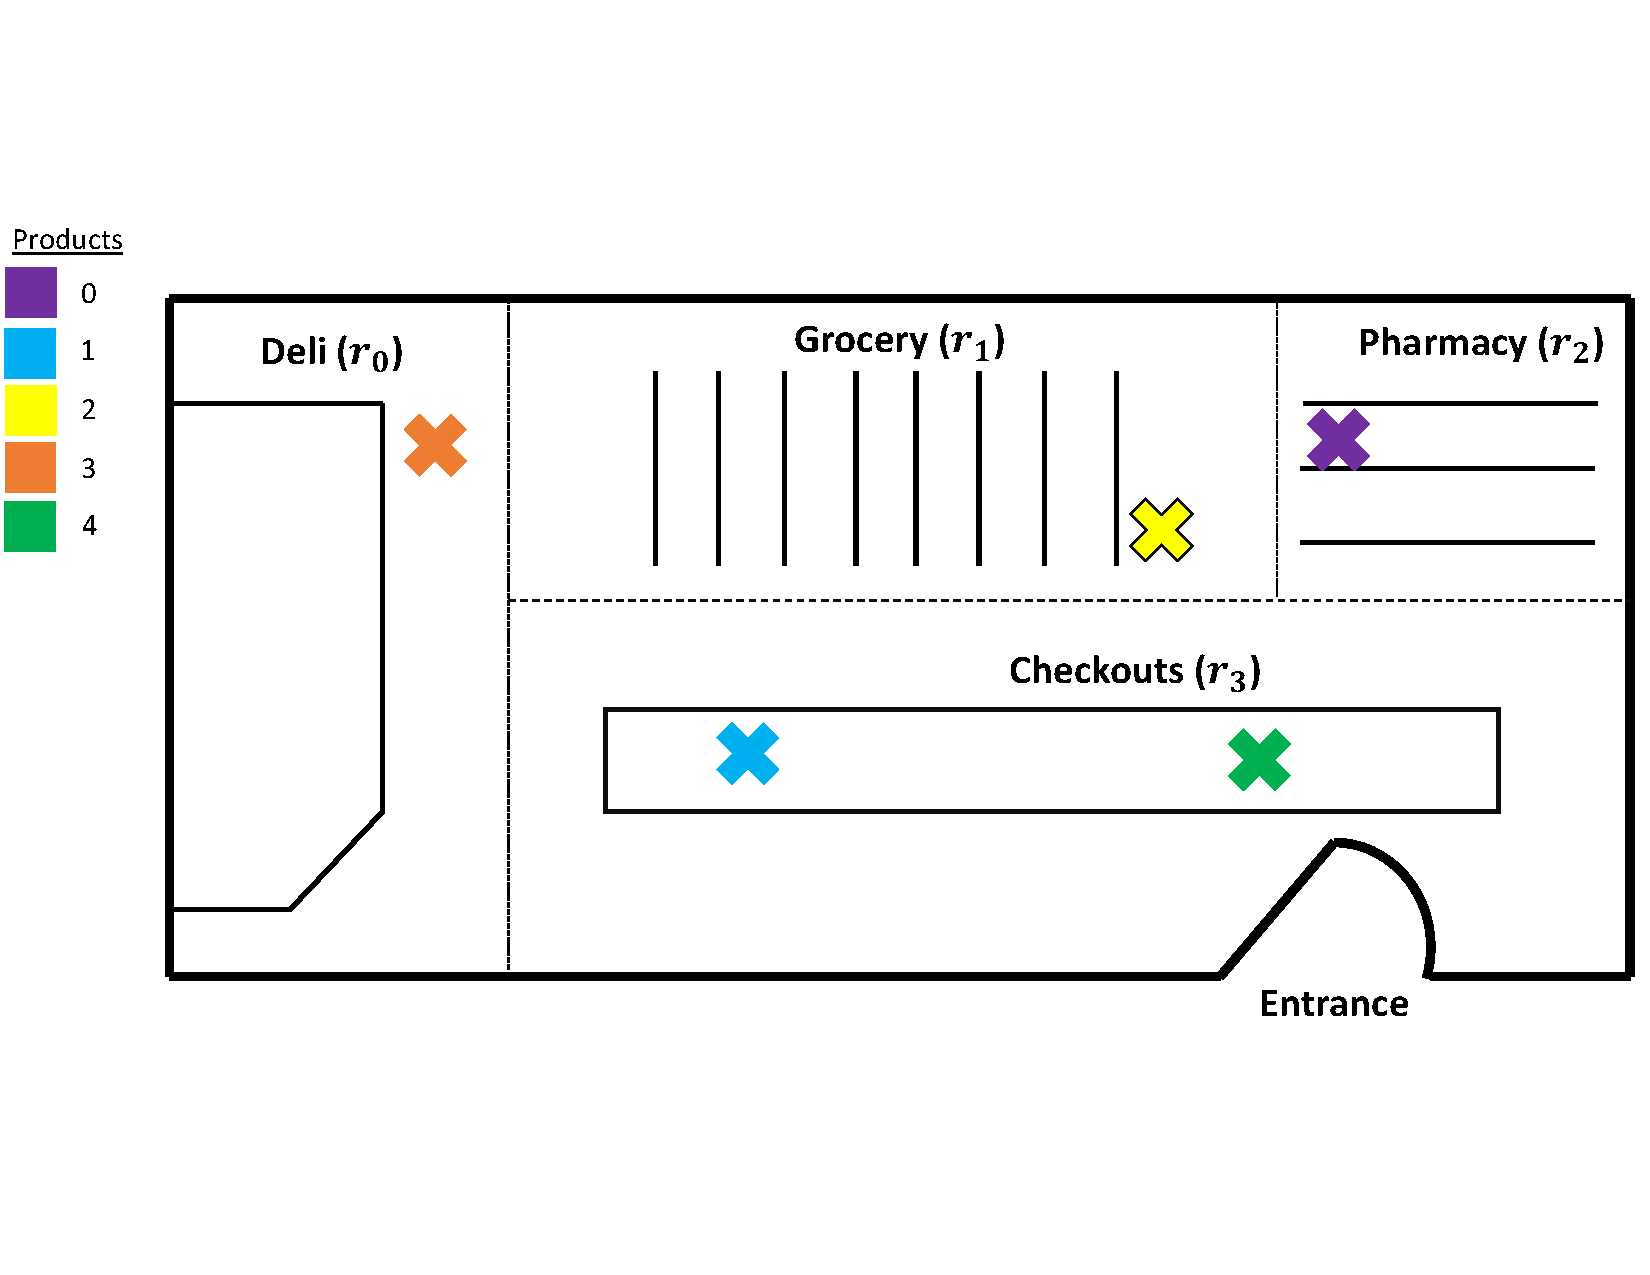
\includegraphics[width=0.8\linewidth]{figs/store-layout.pdf}} \\
\vspace{-4mm}
\subfloat[State matrix]{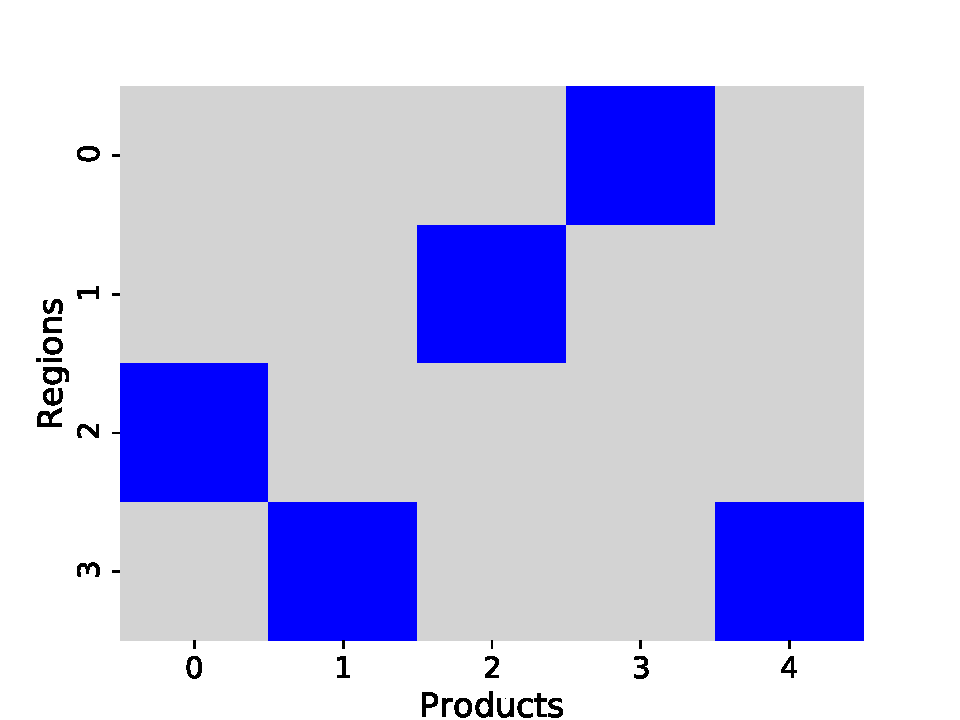
\includegraphics[width=0.5\linewidth]{figs/example-fig-heatmap.pdf}}
\subfloat[Revenue distribution]{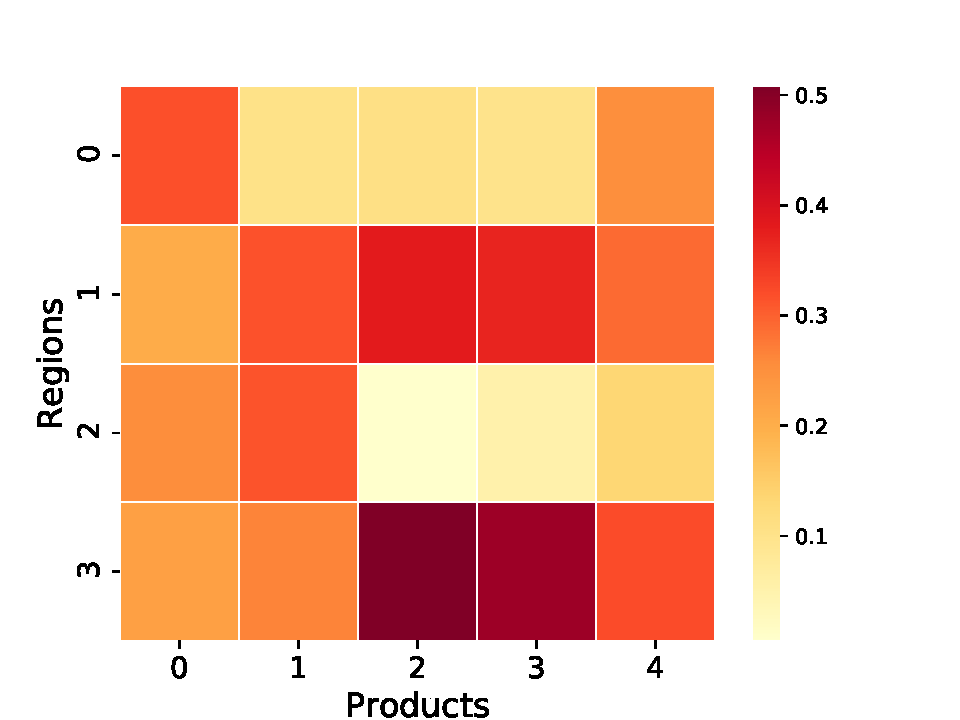
\includegraphics[width=0.5\linewidth]{figs/example-fig-heatmap-sales.pdf}}

\caption{An example of the product allocation problem in physical retail. We provide a sample floor plan of a small, retail environment (a). Each section of the store is partitioned into ``regions''  (e.g., $r_1$). The product distributor or retailer has to choose the regions in which to put each of five possible products. The current product locations are plotted as colored $x$'s. We visualize the current allocation strategy as a state matrix, where blue components denote a given region, product combination has been selected (b). We also show the historical spatial distribution of revenue as a heat map (c). Darker colors indicate more historical revenue. The figure suggests that the current configuration may be sub-optimal. In reality, many large retail environments have thousands of products and many regions.}
\label{intro-fig}
\vspace{-4mm}
\end{figure}



Some existing work explores domains adjacent to the optimal product allocation problem. A large body of operations research analyzes shelf space distribution. For example, early work proposed a dynamic programming algorithm to discover an optimal shelf allocation strategy \cite{zufryden}. Other work poses shelf space allocation as a constrained optimization problem that can be solved via simulated annealing \cite{borin}. More contemporary studies propose frequent pattern mining approaches to determine profitable product item sets \cite{brijs} \cite{aloysius}. To the best of our knowledge, none of the existing literature has studied the spatial effects of product locations across the entire store. 


However, learning a strategy for optimal product allocation is non-trivial. First, the number of candidate allocation strategies is large but the historical data usually only explores a small subset. Not to mention that sales are also correlated with other factors such as holidays and store promotions, which makes the search space even bigger. Because of this issue of data sparsity we cannot directly rely on historical data to learn the best strategy. Second, the cost of experimentation and exploration is high. It is not feasible to perform extensive experiments due to the potential lost revenue and the physical cost of moving products around the store. Finally, the correlation between product positions and sales is likely complex and non-linear due to the dynamic nature of the market; simple search heuristics may not provide an optimal policy. For all of these reasons, we need an approach that can accurately reflect the environment in a cost-efficient way.

Therefore, we design a new framework to solve these challenges. We propose a probabilistic spatial demand simulator to be a mirror of the real environment and act as a mechanism to study more complex search algorithms such as reinforcement learning without incurring the high cost of exploration in the physical world. We train the proposed model using a new, real-world dataset. Additionally, when deployed online, the model could be used to perform Monte Carlo rollouts for efficient exploration and experimentation \cite{kaiser}.


In our experiments, we demonstrate that the proposed model can effectively recover ground truth test data in two retail environments. Finally, we do a preliminary study into different optimization techniques using the proposed model.


In summary the key contributions of our paper are:

\begin{itemize}
    \item We study the new problem of optimal product allocation in physical retail
    \item We propose a probabilistic model of spatial demand that can accurately recover observed data, and generate data for new environment states
    \item We train PSD-sim on real data from two different retail stores
    \item We do a preliminary study into various optimization methods and show that Deep Q-Learning can learn an optimal allocation policy
\end{itemize}

